\documentclass[11pt,a4paper]{article}

% basic packages
\usepackage{float}
\usepackage{fullpage}
\usepackage{polski}
\usepackage{graphicx}
\usepackage[utf8x]{inputenc}

% bibliography and links
\usepackage{url}
\usepackage{cite}
\def\UrlBreaks{\do\/\do-}
\usepackage[hidelinks]{hyperref}

% graphs
\usepackage{tikz}
\usetikzlibrary{arrows}

% listings
\usepackage{listings}
\usepackage{color}
\definecolor{dkgreen}{rgb}{0,0.6,0}
\definecolor{gray}{rgb}{0.5,0.5,0.5}
\definecolor{mauve}{rgb}{0.58,0,0.82}
\lstset{
  basicstyle=\footnotesize,    
  captionpos=b,             
  commentstyle=\color{dkgreen},  
  frame=single,       
  keywordstyle=\color{blue},  
  language=Python,   
  numbers=left,     
  numbersep=7pt,   
  numberstyle=\tiny\color{gray}, 
  rulecolor=\color{black},  
  stringstyle=\color{mauve}, 
  tabsize=2,    
  title=\lstname
}

\begin{document}

\begin{titlepage}
  \begin{center}

    \textsc{\Large Politechnika Warszawska}\\[0.1cm]
    \small Wydział Elektroniki i Technik Informacyjnych
    \vfill

    \textsc{\small Wprowadzenie do Eksploracji Danych Tekstowych w Środowisku WWW }\\[0.1cm]
    \Huge Gromadzenie i~przechowywanie przepisów kulinarnych przy użyciu ontologii\\[1.5cm]
    \small Sprawozdanie końcowe\\[2.5cm]

    \vfill

    \begin{minipage}{0.4\textwidth}
      \begin{flushleft} \large
        \emph{Autorzy:}\\[0.1cm]
        Maciej \textsc{Suchecki}\\
        Michał \textsc{Toporowski}\\
        Jacek \textsc{Witkowski}\\
      \end{flushleft}
    \end{minipage}
    \begin{minipage}{0.4\textwidth}
      \begin{flushright} \large
        \emph{Prowadzący:}\\[0.1cm]
        dr~inż.~Piotr \textsc{Andruszkiewicz}\\[1cm]
      \end{flushright}
    \end{minipage}

    \vfill
    {\large \today}

  \end{center}
\end{titlepage}

\section{Treść zadania}
\paragraph{Tytuł} Gromadzenie i przechowywanie przepisów kulinarnych w ustrukturalizowany sposób, przy użyciu ontologii.
\paragraph{Opis}
\begin{itemize}
  \item ekstrakcja informacji ze stron z przepisami (Information Extraction)
  \item odwzorowanie wyekstrahowanych elementów na ontologię
  \item wstawienie instancji do ontologii/ew. modyfikacja ontologii (na poziomie pojęć, dodanie nowych pojęć)
  \item wykonywanie zapytań na ontologii
\end{itemize}

\section{Definicja problemu}
Przepisy kulinarne są dostępne w~ogromnych ilościach w~Internecie. Znalezienie interesujących nas przepisów jest bardzo owocne, bez względu na zdefiniowane wymagania -- takie jak język przepisu, czy składniki potrzebne do jego wykonania. Z~drugiej jednak strony, przepisy te są udostępniane w~sposób silnie nieustruktruralizowany, a~zatem poruszanie się w~takim zbiorze oraz pobieranie z~niego informacji staje się żmudne i~trudne. Z~tego powodu problem ekstrakcji wspomnianych przepisów z~sieci Internet oraz ich przechowywanie w~ustrukturalizowany sposób wydaje się ciekawy oraz ważny.

\section{Opis rozwiązania}
Rozwiązaniem tak postawionego problemu będzie program eksplorujący przepisy kulinarne znajdujące się w~sieci Internet. Będzie on pobierał przepisy z~wcześniej zdefiniowanych stron WWW. Ich lista będzie zdefiniowana w~pliku tekstowym, przy czym nie będzie ona modyfikowalna przez użytkownika, z~racji na konieczność definiowania różnych fragmentów kodu w~zależności od struktury badanej strony. Moduły aplikacji, które będą brały udział w~początkowej analizie przepisów będą silnie zależne od układu badanych stron z~przepisami. Ponadto, dla każdej strony będzie zdefiniowana liczba przepisów, którą program ma z~danej strony odczytać. Wartość ta będzie mogła być modyfikowana przez użytkownika.\\

Podczas działania programu wczytane przepisy będą poddawane działaniu procesora języka naturalnego, odwzorowywane na wcześniej zdefiniowaną ontologię, oraz wstawiane do niej jako nowe instancje. Wynikiem działania programu będzie wypełniona przepisami grafowa baza danych. Będzie można wykonywać na niej zapytania, pozwalające na ekstrakcję z~niej ustrukturalizowanych danych przepisów.

\section{Implementacja}
Program będzie napisany w~języku Python i~będzie składał się z~czterech modułów, widocznych na poniższym rysunku:\\


\begin{tikzpicture}[shorten >=1pt,->,draw=black!50, node distance=\layersep]
  \tikzstyle{every pin edge}=[<-,shorten <=1pt]
  \tikzstyle{module}=[rectangle,draw,minimum size=17pt,inner sep=2pt]

  \node[module, pin=left:WWW] (crawler) at (0,-1) {WebScraper};
  \node[module] (parser) at (2.5,-1) {HTMLParser};
  \path (crawler) edge (parser);
  \node[module] (processor) at (5.5,-1) {NLProcessor};
  \path (parser) edge (processor);
  \node[module, pin={[pin edge={->}]right:Baza danych}] (connector) at (8.5,-1) {GraphDatabase};
  \path (processor) edge (connector);
\end{tikzpicture}

Opis każdego z~modułów znajduje się w~kolejnych podrozdziałach.

\subsection{Moduł \textit{WebScraper}}
\subsubsection{Wejście}
Moduł będzie pobierał z~pliku listę adresów stron, z których powinien pobrać przepisy -- wraz z~liczbą przepisów do pobrania z~każdej strony.
\subsubsection{Sposób działania oraz wykorzystywane biblioteki}
Z pomocą bibliotek \textit{requests} oraz \textit{BeautifulSoup} moduł będzie pobierał cały kod HTML dotyczący przepisu, zapisując go w~strukturze \textit{RawRecipe}.
\subsubsection{Wyjście}
Wynikiem działania modułu \textit{WebScraper} -- przekazywanym do modułu \textit{HTMLParser}, będzie zbiór obiektów typu \textit{RawRecipe}, zawierających adres WWW przepisu, oraz jego kod HTML zawierający wszystkie dane jego dotyczące -- takie, jak opis, nazwa, składniki itp.

\subsection{Moduł \textit{HTMLParser}}
\subsubsection{Wejście}
Moduł będzie przyjmował zbiór obiektów typu \textit{RawRecipe}, przekazanych mu od modułu \textit{WebScraper}.
\subsubsection{Sposób działania oraz wykorzystywane biblioteki}
Za pomocą biblioteki \textit{BeautifulSoup} -- służącej do parsowania dokumentów HTML -- moduł będzie starał się wyekstrahować jak najwięcej przydatnych informacji dotyczących struktury przepisu z~otrzymanego kodu HTML.
\subsubsection{Wyjście}
Wynikiem działania modułu \textit{HTMLParser} -- przekazywanym do modułu \textit{NLProcessor}, będzie zbiór obiektów typu \textit{ParsedRecipe}, zawierających pola:
\begin{itemize}
  \item \textbf{url} -- pole zawierające dokładny adres URL przepisu na stronie WWW
  \item \textbf{name} -- pole zawierające nazwę przepisu
  \item \textbf{ingredients} -- pole zawierające listę napisów opisujących poszczególne składniki przepisu (wraz z~podanymi ilościami)
  \item \textbf{preparation} -- pole zawierające właściwy tekst przepisu -- inaczej, sposób przygotowywania danej potrawy
  \item \textbf{additional\_attributes} -- opcjonalne pole, zawierające słownik dodatkowych atrybutów, takich jak: czas przygotowywania, stopień trudności itp. Możliwe klucze dla słownika będą z~góry zdefiniowane w~programie.
\end{itemize}

\newpage
\subsection{Moduł \textit{NLProcessor}}
\subsubsection{Wejście}
Moduł będzie przyjmował zbiór obiektów typu \textit{ParsedRecipe}, przekazanych mu od modułu \textit{HTMLParser}.
\subsubsection{Sposób działania oraz wykorzystywane biblioteki}
Za pomocą biblioteki \textit{NLTK} moduł będzie przekształcał tekst opisujący składniki przepisu na model obiektowy.\\ 

W ramach tego procesu wykonywane będą czynności takie, jak:
\begin{itemize}
	\item lematyzacja 
	\item filtrowanie słów nieistotnych
	\item wyodrębnienie z tekstu informacji o nazwach składników i ich ilości
	\item zbudowanie powiązań pomiędzy krokami przepisu a wykorzystywanymi składnikami
\end{itemize}
\subsubsection{Wyjście}
Wynikiem działania modułu \textit{NLProcessor} -- przekazywanym do modułu \textit{GraphDatabase}, będzie zbiór obiektów typu \textit{ProcessedRecipe}, zawierających pola:
\begin{itemize}
  \item \textbf{url} -- pole zawierające dokładny adres URL przepisu na stronie WWW
  \item \textbf{name} -- pole zawierające nazwę przepisu
  \item \textbf{additional\_attributes} -- opcjonalne pole, zawierające słownik dodatkowych atrybutów, takich jak: czas przygotowywania, stopień trudności itp. Możliwe klucze dla słownika będą z~góry zdefiniowane w~programie.
  \item \textbf{ingredients} -- pole zawierające zbiór składników w postaci obiektów zawierających następujące pola:
  \begin{itemize}
    \item \textbf{name} -- nazwa składnika
    \item \textbf{amount} -- ilość składnika (obiekt zawierający wartość oraz jednostkę)
  \end{itemize}
  \item \textbf{preparation} - pole zawierające zbiór obiektów \textit{PreparationStep} zawierających następujące pola:
    \begin{itemize}
    \item \textbf{text} -- opis kroku
    \item \textbf{ingredients} -- lista składników wykorzystywanych w danym kroku
  \end{itemize}
\end{itemize}

\subsection{Moduł \textit{GraphDatabase}}
\subsubsection{Wejście}
Moduł będzie przyjmował zbiór obiektów typu \textit{ProcessedRecipe}, przekazanych mu od modułu \textit{NLProcessor}.
\subsubsection{Sposób działania oraz wykorzystywane biblioteki}
Za pomocą biblioteki \textit{rdflib} oraz zdefiniowanej przez autorów ontologii, moduł utworzy z~przepisów grafową bazę danych. Po zachowaniu wszystkich przepisów, baza danych będzie zachowana w~pliku o~formacie \textit{RDF}, aby można było wykonywać na niej zapytania.
\subsubsection{Wyjście}
Wynikiem działania modułu będzie grafowa baza danych zapisana w~pliku. Do bazy będzie można się odwoływać poprzez zapytania predefiniowane w~skrypcie języka \textit{Python}.

\section{Ontologia}
Na potrzeby projektu została stworzona następująca ontologia ro (Recipe Ontology):
\begin{figure}[H]
  \centering
  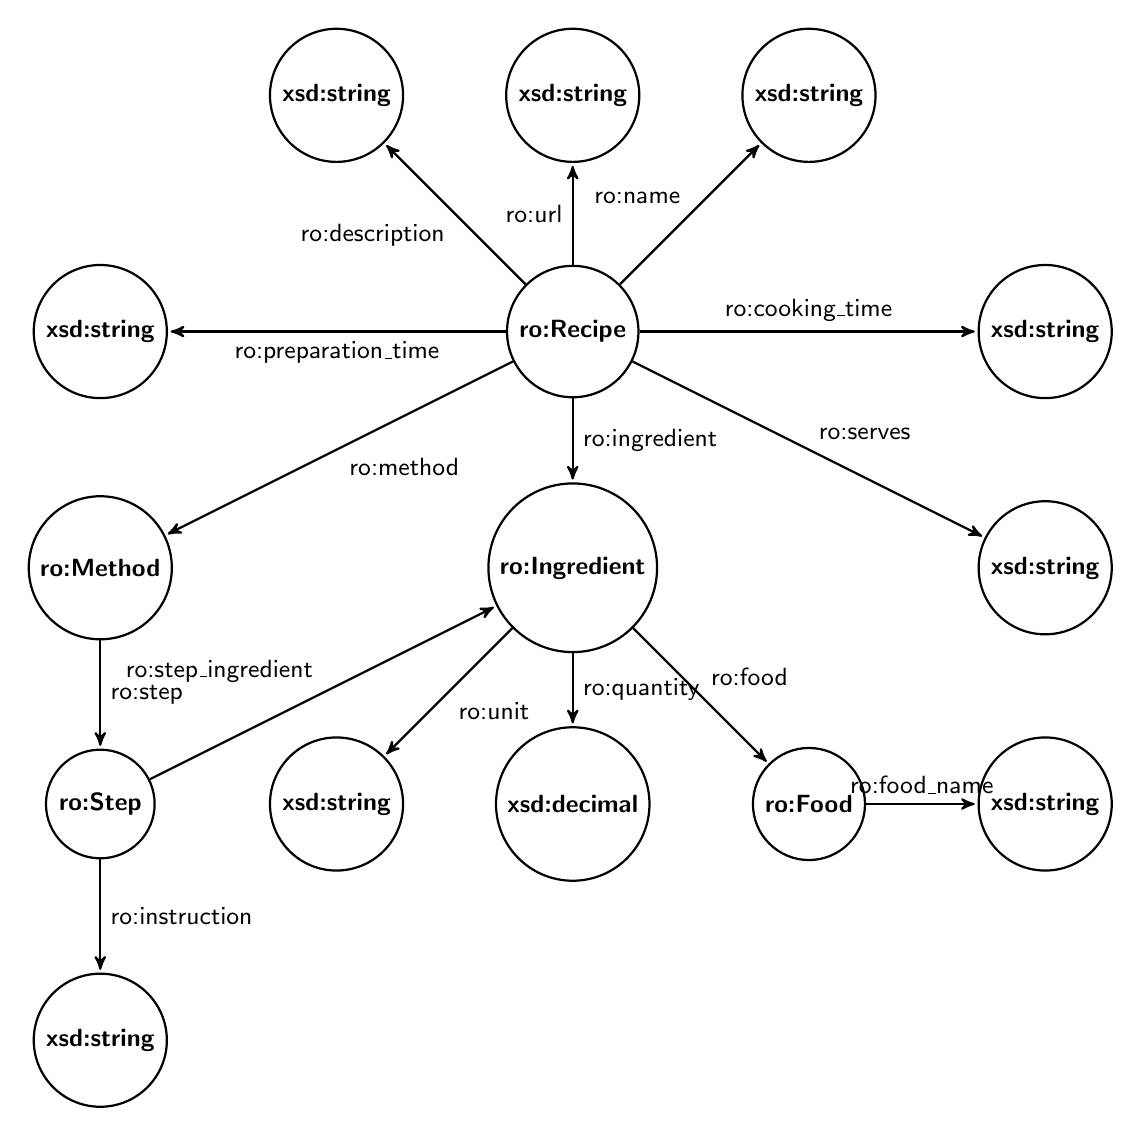
\begin{tikzpicture}[->,>=stealth',shorten >=1pt,auto,node distance=3cm,
    thick,main node/.style={circle,draw,font=\sffamily\bfseries\small}]

    \node[main node] (0) {ro:Recipe};

    % Ingredients and below
    \node[main node] (1) [below of=0] {ro:Ingredient};
    \node[main node] (2) [below of=1] {xsd:decimal};
    \node[main node] (3) [right of=2] {ro:Food};
    \node[main node] (4) [right of=3] {xsd:string};
    \node[main node] (5) [left of=2] {xsd:string};

    % Method and Steps
    \node[main node] (6) [left of=5] {ro:Step};
    \node[main node] (7) [above of=6] {ro:Method};
    \node[main node] (8) [below of=6] {xsd:string};

    % Recipe attributes
    \node[main node] (9) [above of=0] {xsd:string};
    \node[main node] (10) [left of=9] {xsd:string};
    \node[main node] (11) [right of=9] {xsd:string};
    \node[main node] (12) [above of=7] {xsd:string};
    \node[main node] (13) [above of=4] {xsd:string};
    \node[main node] (14) [above of=13] {xsd:string};

    \path[every node/.style={font=\sffamily\small}]
    % Recipe connections
    (0) edge node {ro:name} (11)
    edge node {ro:url} (9)
    edge node {ro:serves} (13)
    edge node {ro:description} (10)
    edge node {ro:preparation\_time} (12)
    edge node {ro:cooking\_time} (14)
    edge node {ro:ingredient} (1)
    edge node {ro:method} (7)
    % Ingredient connections
    (1) edge node {ro:food} (3)
    edge node {ro:quantity} (2)
    edge node {ro:unit} (5)
    (3) edge node {ro:food\_name} (4)
    % Method and Step connections
    (7) edge node {ro:step} (6)
    (6) edge node {ro:step\_ingredient} (1)
    (6) edge node {ro:instruction} (8);
  \end{tikzpicture}
  \caption{Ontologia utworzona na potrzeby projektu.}
  \label{figure:ontology}
\end{figure}

Została ona wykorzystana do zapisywania przepisów w~bazie danych. Plik z~definicją ontologii w~formacie \textit{Turtle} znajduje się pod ścieżką \textit{rextractor/db/recipes\_ontology.ttl}.

\newpage
\section{Instrukcja obsługi}
\subsection{Uruchomienie programu}
Aby uruchomić program, należy zainstalować interpreter języka Python w~wersji 3\footnote{\url{https://www.python.org/downloads/}} oraz program pip\footnote{\url{https://pip.pypa.io/en/latest/installing.html}}. Następnie należy sklonować projekt, zainstalować zależności oraz uruchomić aplikację za pomocą następujących komend:\\

\begin{lstlisting}
$ git clone git@github.com:mc-suchecki/Rextractor.git
$ cd Rextractor
$ pip install -r requirements.txt
$ python rextractor.py
\end{lstlisting}

W~wyniku ww. operacji w~katalogu głównym aplikacji zostanie utworzony plik \textit{recipes.rdf} zawierający przepisy zapisane w~formacie RDF. Domyślnie program pobiera przepisy tylko z~pierwszych stron dla adresów: \textit{www.simplyrecipes.com} oraz \textit{www.eatingwell.com}. Oczywiście, program jest w~stanie pobrać wszystkie przepisy dostępne na ww. stronach. Liczbę obsługiwanych stron z~przepisami można łatwo zwiększyć.

\subsection{Wykonywanie przykładowych zapytań}
Po utworzeniu pliku \textit{recipes.rdf} można już wykonywać przykładowe zapytania na stworzonej bazie. Aby to uczynić, należy w~katalogu aplikacji wywołać polecenie \textit{python query.py} które uruchomi prosty program do wykonywania predefiniowanych zapytań. Aby wykonać jedno z~nich, wystarczy podać numer zapytania i~wcisnąć Enter. Program działa w~pętli nieskończonej -- w~celu wyjścia należy wpisać pustą linię. Na chwilę obecną zdefiniowane są 3 przykładowe zapytania, opisane w~poniższych fragmentach dokumentacji.

\subsubsection{Wypisanie dostępnych przepisów}
\begin{lstlisting}
$ python query.py
Here are possible queries:
0. List all imported recipes
1. List all imported ingredients
2. List all recipes containing desired ingredient

Please input query number (blank line exits): 0

Executing query number 0...
Ancho-Honey Pork Tenderloin with Cheese Grits
Baked Parmesan Chicken Nuggets
Beef & Portobello Mushroom Stroganoff
Black Bean Nacho Pizza
Broccoli Cheddar Mac and Cheese
Brussels Sprouts with Toasted Almonds
Caramelized Onion & White Bean Flatbread
...
$
\end{lstlisting}

\subsubsection{Wypisanie dostępnych składników}
\begin{lstlisting}
$ python query.py
Here are possible queries:
0. List all imported recipes
1. List all imported ingredients
2. List all recipes containing desired ingredient

Please input query number (blank line exits): 1

Executing query number 1...
balsam vinegar
bean
black pepper
blue chees
bread
broccoli
butter
canola oil
carrot
...
$
\end{lstlisting}

\subsubsection{Wypisanie przepisów zawierających dany składnik}
\begin{lstlisting}
$ python query.py
Here are possible queries:
0. List all imported recipes
1. List all imported ingredients
2. List all recipes containing desired ingredient

Please input query number (blank line exits): 2    
Ingredient name: onion

Brussels Sprouts with Toasted Almonds
Cioppino
Cumin-Scented Wheat Berry-Lentil Soup
Curried Turkey Soup
How to Chop an Onion
Quinoa Lasagna

Here are possible queries:
0. List all imported recipes
1. List all imported ingredients
2. List all recipes containing desired ingredient

Please input query number (blank line exits): 2
Ingredient name: pepper

Brussels Sprouts with Toasted Almonds
Cioppino
Moms Turkey Soup
Swedish Meatballs
$
\end{lstlisting}

%\subsubsection{Wypisanie przepisów, które da się zrealizować z~listy podanych składników}

\newpage
\section{Testy}
\subsection{Testy end-to-end}
Testy end-to-end polegają na uruchomieniu całego procesu od pobrania przepisów z sieci, poprzez parsowanie i~przetwarzanie języka naturalnego, aż po zapis do grafowej bazy danych. Pliki testujące znajdują się w~folderze \textit{tests}.

\subsection{Testy modułu \textit{NLProcessor}}
Do modułu NLProcessor zostały utworzone testy weryfikujące poprawność wydobywania danych z tekstu w języku naturalnym. Testy zostały wykonane w następujący sposób:
\begin{itemize}
\item jako dane wejściowe zostały przekazane obiekty typu \textit{ParsedRecipe} 
\item zdefiniowano oczekiwany wynik przetworzenia danych przepisów (w postaci obiektów typu \textit{ProcessedRecipe})
\item uruchomiono moduł NLProcessor z danymi parametrami wejściowymi i zweryfikowano, czy wynik jest zgodny z oczekiwanym.  
\end{itemize}
\paragraph{Wynik} 
Dla testowanych przepisów, 78\% składników zostało przetworzonych całkowicie zgodnie z oczekiwaniami tj. każdy element listy składników miał identyczną nazwę, ilość oraz jednostkę, jak w danych oczekiwanych.\\
W pozostałych przypadkach zaobserwowano następujące niezgodności:
\begin{enumerate}
\item została wydobyta jedynie część nazwy składnika (np. \textit{fillet} zamiast \textit{salmon fillet})
\item część nazwy składnika została sklasyfikowana jako nazwa jednostki lub vice versa
\item rozpoznano dany fragment tekstu jako opis jednego składnika, gdy w rzeczywistości zawierał opis dwóch
\end{enumerate}
Przyczyny problemów:
\begin{itemize}
\item niepoprawna klasyfikacja części mowy przez bibliotekę NLTK w niektórych zdaniach
\item płynność i różnorodność języka naturalnego utrudniająca przewidzenie struktury tekstu
\end{itemize}
Warto jednak zauważyć, że pomimo powyższych problemów, zdania o typowej strukturze są przetwarzane na ogół dobrze, zaś niezgodności typu 1. i 3. zazwyczaj nie dyskwalifikują wyniku tj. może być on w dalszym ciągu użyteczny.

\subsection{Wydajność}


\newpage
\section{Wnioski}
Podczas tworzenia oraz testowania programu doszliśmy do następujących wniosków:

\begin{itemize}
  \item Python świetnie się nadaje do procesowania tekstu, web scrapingu itp.
  \item Narzędzia z biblioteki \textit{NTLK} znacznie ułatwiają przetwarzanie języka naturalnego w Pythonie, jednak nie są idealne i czasem produkują niepoprawne wyniki.
  \item Słabe wsparcie dla ontologii i OWL dla Pythona.
  \item Implementacja aplikacji wydobywającej wiedzę ze stron webowych wymaga dostosowania do konkretnej strony i konkretnego stylu.
\end{itemize}

\subsection{Ewentualne zastosowania aplikacji}
Po zastanowieniu, byliśmy w~stanie wymienić następujące propozycje zastosowania aplikacji w~praktyce:
\begin{itemize}
  \item jako generator zawartości dla strony z przepisami
  \item jako narzędzie dla dietetyka (wykonywanie zapytań -- np. znajdź przepis wykorzystujący pomidory)
  \item jako narzędzie pomagające odpowiedzieć na pytanie "Co można zrobić ze składników znajdujących się aktualnie w lodówce?"
\end{itemize}

\subsection{Rozwój aplikacji}
Architektura aplikacji wspiera jej rozbudowę. Ma ona wiele możliwych dróg rozwoju, takich jak:

\begin{itemize}
  \item implementacja obsługi kolejnych stron z~przepisami
  \item modyfikacja klasy WebScraper w~celu uzyskania wielowątkowej pracy -- znacznie większa wydajność
  \item zastosowanie innej bazy danych -- np. relacyjnej
  \item można pokusić się o mechanizm zapobiegający ponownego wstawiania istniejących przepisów -- wtedy można uruchamiać aplikację cyklicznie jako crawler
\end{itemize}

Ponadto, jakość kodu została zapewniona poprzez stosowanie się do standardu PEP8 oraz stosowania narzędzia pylint. Kod był regularnie analizowany tym narzędziem -- gotowy projekt uzyskał ocenę 8.17/10.

\section{Podsumowanie}
Praca nad projektem była dla nas ciekawa i~rozwijająca, z~wielu powodów. Po pierwsze, mieliśmy okazję poznać język Python -- jak pisze się w~nim większe aplikacje obiektowe. Poza tym, zdobyliśmy wiedzę nt. procesowania tekstu, web scrapingu oraz ontologii.

% bibliography
%\addcontentsline{toc}{chapter}{Literatura}
%\bibliography{references}{}
%\bibliographystyle{alpha}

\end{document}
